\section{Prototype interviews}\label{section:interview2}
State of the art undersøgelsen på \myref{s:SOTA} viste, at der er forskellige løsninger.
Ingen af løsningerne tager tilbud fra alle butikker, har indkøbsliste, tilbyder opskrifter, der er integreret med tilbudene, samt vurdering af disse.
Derfor har vi udformet en prototype i Microsoft Office Powerpoint, som viser, hvordan de forskellige funktionaliteter kunne se ud.
Diasshowet består af forskellige skærmbilleder, der kan navigeres imellem ved tryk på de gule felter.

Et eksempel kan ses på \myref{ss:Prototype}.

\begin{wrapfigure}{o}{0.68\textwidth}
\vspace{-20pt}
	\begin{center}
		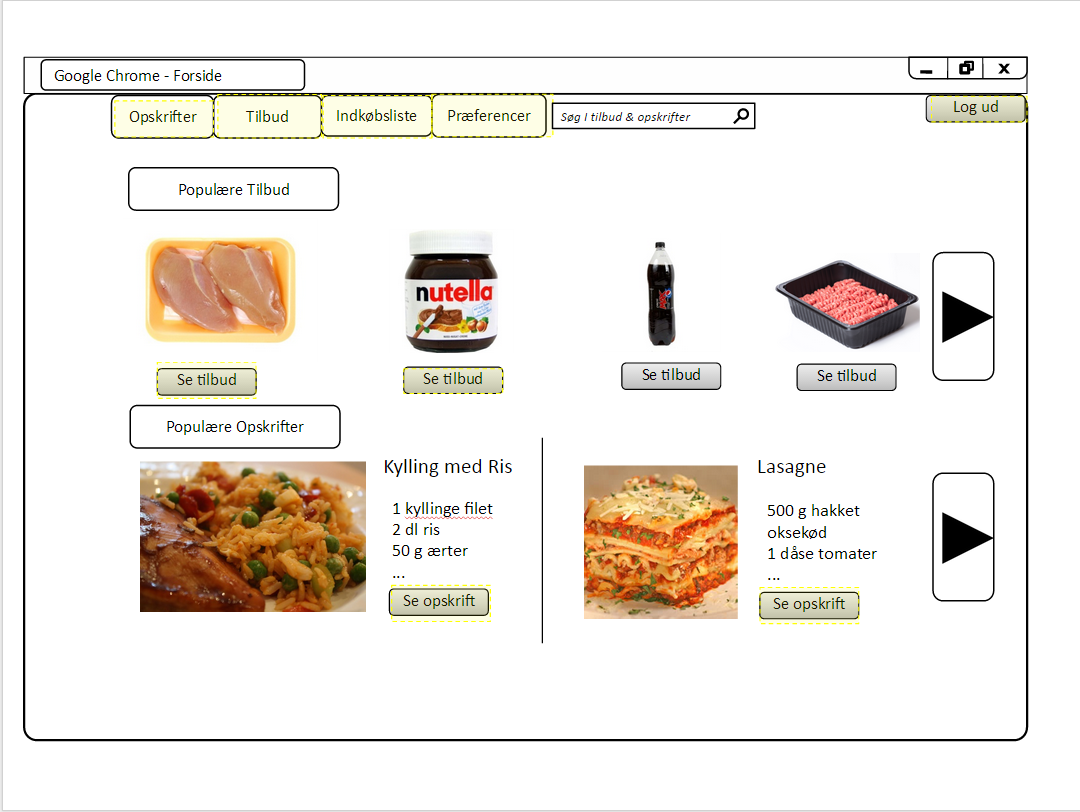
\includegraphics[width=0.66\textwidth]{images/Images/prototype-forside.PNG}
	\end{center}
	\vspace{-20pt}
	\caption{Forside fra Prototypen der blev brugt i forbindelse med vores 2. runde af interviews.}\label{ss:Prototype}
	\vspace{-20pt}
\end{wrapfigure}

Prototypen bruges i vores 2. runde af interviews, som har til formål at forstå, hvilke funktionaliteter potentielle brugere ønsker i en løsning.
Aldersgruppen for de interviewede lå mellem 20-49.

Den 2. runde af interviews blev udført som semi-strukturerede interviews, med personer der var oprettet kontakt med på forhånd, frem for at finde fremmede på gaden.
Dette tillod os, at interviewe i længere tid, og betød at de interviewede i forvejen var forberedt på et interview.
Et semi-struktureret interview tillader, at der afviges fra de nedskrevne spørgsmål for at følge samtalen og stille uddybende spørgsmål omkring potentielle kommentarer.\cite[s. 142-146]{DIS2014}
 
Spørgsmålene var lavet med det formål at få indblik i deres tanker omkring et system, inden de blev præsenteret for de idéer, der ellers var omkring systemet.
For at opnå dette blev de først præsenteret for et spørgsmål, som hvilke opgaver de mente systemet kunne behjælpe, hvorefter der blev uddybet, hvorfor præcis disse funktionaliteter blev nævnt af de interviewede.
Først efter at have fået deres idéer, blev de præsenteret for idéer projektgruppen havde opnået, og herefter reflekterede de over hvorfor nogle ikke var nævnt, samt hvad de mente om disse forslag.
Et dokument over de strukturerede spørgsmål af interview-sessionerne, kan findes i \myref{ch:PrototypeInterview}.
Ud fra responsen opsamlet gennem undersøgelsen, vurderer vi, at en løsning bør have følgende funktionaliteter:

\begin{itemize}[nolistsep,noitemsep]
	\item Indkøbsliste integreret med tilbud.
	\item Oversigt over tilbud fra samtlige dagligvarebutikker.
	\item Mulighed for at vurdere opskrifterne og få anbefalet lignende.
	\item Valg af hvor man vil handle, hvilke madvarer man ikke vil spise osv.
	\item Deling af indkøbsliste med andre.
	\item Overvågning af varer, så man får en besked, hvis noget kommer på tilbud.
\end{itemize}

Der var også andre funktionaliteter, som nogle af de adspurgte foreslog, kunne laves for systemet.
Disse er dog blevet fravalgt, enten fordi det kun var enkelte, der bakkede op omkring funktionen, eller fordi det ikke passede ind med systemets anden funktionalitet.
F.eks. blev en kalorietæller foreslået af en af de adspurgte, men dette vælges der at afgrænse fra, da det ikke hænger så godt sammen med resten af den meget tilbudsorienterede løsning.

Herudover gav de interviewede også forslag og ønsker angående hvilke funktionaliteter, der skulle være hvor i et desktop layout.
Disse forslag tages med i overvejelserne, når brugergrænsefladen skal designes.
En oversigt over de adspurgtes svar samt forslag, kan ses i \myref{ch:protorespons}.
